\subsection{Burnside's Lemma}
Burnside’s lemma can be used to count the number of combinations so that
only one representative is counted for each group of symmetric combinations.
For example, if we have a necklace with different colored pearls and we want to know
how many different combinations we can make.

For example, if we have a necklace colored like this:

\begin{center}
    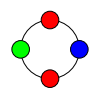
\includegraphics[scale=.6, keepaspectratio]{./Theory/images/burnside1.png}
\end{center}

This variations are the same if we consider that we can rotate the necklace:

\begin{center}
    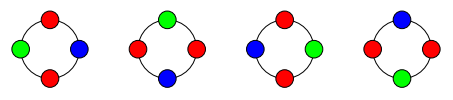
\includegraphics[scale=.6, keepaspectratio]{./Theory/images/burnside2.png}
\end{center}

When the number of steps is k, the number of necklaces that remain the same are:
$$ m^{gcd(k, n)} $$

The number of diferent combinations for m colors and a necklace of size n is 
$$ \sum_{i=0}^{n - 1} \dfrac{m^{gcd(i, n)}}{n} $$

So a necklace of length 4 with 3 colors has
$$ \dfrac{3^{4} + 3 + 3^{2} + 3}{4} = 24 $$